\documentclass[aspectratio=169,10pt]{beamer}

\usetheme{Madrid}
\usecolortheme{default}
\usefonttheme{professionalfonts}

\usepackage[T1]{fontenc}
\usepackage[utf8]{inputenc}
\usepackage{lmodern}
\usepackage{amsmath,amssymb,bm}
\usepackage{booktabs}
\usepackage{tikz}
\usetikzlibrary{arrows.meta,positioning,fit,calc}

\definecolor{JHUBlue}{RGB}{0,45,114}
\definecolor{JHUGold}{RGB}{207,181,59}
\definecolor{SoftRed}{RGB}{176,55,55}
\definecolor{SoftGreen}{RGB}{48,128,88}
\definecolor{SoftGray}{RGB}{90,96,104}

\setbeamercolor{structure}{fg=JHUBlue}
\setbeamercolor{frametitle}{fg=white,bg=JHUBlue}
\setbeamercolor{title}{fg=white,bg=JHUBlue}
\setbeamercolor{block title}{fg=white,bg=JHUBlue}
\setbeamercolor{block body}{bg=black!3}
\setbeamertemplate{navigation symbols}{}
\setbeamertemplate{itemize items}[circle]

\newcommand{\Deq}{D_{\mathrm{eq}}}
\newcommand{\Dne}{D_{\mathrm{NE}}}
\newcommand{\Edft}{E_{\mathrm{DFT}}}
\newcommand{\Fdft}{F_{\mathrm{DFT}}}
\newcommand{\EM}{E_M}
\newcommand{\FM}{F_M}
\newcommand{\Gdft}{\Gamma_{\mathrm{DFT}}^\star}
\newcommand{\GM}{\Gamma_M^\star}
\newcommand{\Ea}{E_{\mathrm{a}}}
\newcommand{\epsfixed}{\varepsilon_{\mathrm{fixed}}}
\newcommand{\epsself}{\varepsilon_{\mathrm{self}}}
\newcommand{\epsreport}{\varepsilon_{\mathrm{report}}}
\newcommand{\dpath}{d_{\mathrm{path}}}

\title[Non-Equilibrium Probes for MLFFs]{Non-Equilibrium Migration Probes as a Task-Relevant Benchmark for MLFFs}
\subtitle{Revision 1 walkthrough: scientific pitch, reviewer challenges, and executable closure plan}
\author{Yi Cao, Peter Mastracco, Paulette Clancy}
\institute{Johns Hopkins University}
\date{Revision working deck}

\begin{document}

\begin{frame}
  \titlepage
\end{frame}

\begin{frame}{One-Sentence Pitch}
  \begin{block}{Core thesis}
  The bottleneck in MLFF evaluation is not equilibrium accuracy alone, but robustness under distribution-shifted, non-equilibrium migration probes.
  \end{block}

  \vspace{0.4cm}
  \[
  \text{Good model for deployment}
  \;\not\equiv\;
  \min_M \mathrm{RMSE}_{\Deq}(M)
  \]

  \[
  \text{Good model for migration}
  \;\equiv\;
  \min_M \mathcal{R}_{\Dne}(M)
  \]

  \vspace{0.25cm}
  where $\mathcal{R}_{\Dne}$ measures barrier fidelity, self-consistent path stability,
  path geometry, and long-range mechanical response.
\end{frame}

\begin{frame}{Why This Is Not Just ``Which MLFF Is Better''}
  \begin{columns}[T]
    \begin{column}{0.48\textwidth}
      \begin{block}{Traditional evaluation}
      \[
      \min_\theta
      \mathbb{E}_{(x,y)\sim \Deq}
      \left[
        \ell(f_\theta(x),y)
      \right]
      \]
      \begin{itemize}
        \item relaxed or thermal structures
        \item energy/force RMSE
        \item local interpolation quality
      \end{itemize}
      \end{block}
    \end{column}
    \begin{column}{0.48\textwidth}
      \begin{block}{Real migration task}
      \[
      \mathbb{E}_{(x,y)\sim \Dne}
      \left[
        \ell(f_\theta(x),y)
      \right]
      \]
      \begin{itemize}
        \item high-energy intermediate images
        \item transition-state neighborhoods
        \item long-range strain and sliding
      \end{itemize}
      \end{block}
    \end{column}
  \end{columns}

  \vspace{0.35cm}
  \[
  \Deq \neq \Dne
  \quad\Rightarrow\quad
  \mathrm{RMSE}_{\Deq}(M) \text{ is an insufficient proxy for deployment fidelity.}
  \]
\end{frame}

\begin{frame}{Formal Benchmark Object}
  Define a migration-probe task as
  \[
  \tau = (S, a_m, x_0, x_1, \Gamma, C, R),
  \]
  where
  \begin{itemize}
    \item $S$: host material and cell,
    \item $a_m$: migrating species or local defect coordinate,
    \item $x_0,x_1$: endpoint sites,
    \item $\Gamma=\{X_i\}_{i=0}^{n-1}$: ordered path/images,
    \item $C$: calculator settings, pseudopotentials, cutoffs, k-points,
    \item $R$: relaxation and convergence protocol.
  \end{itemize}

  \vspace{0.2cm}
  The benchmark is a collection
  \[
  \mathcal{T}=\{\tau_1,\ldots,\tau_K\}, \qquad
  \Dne = \bigcup_{\tau\in\mathcal{T}}\{X_i^{(\tau)}\}_{i=0}^{n_\tau-1}.
  \]
\end{frame}

\begin{frame}{The DFT Reference Is Not Just A Number}
  The DFT reference barrier is tied to a path and a convergence protocol:
  \[
  \Delta E_{\mathrm{DFT}}(\Gdft)
  =
  \max_i \Edft(X_i^\star)-\Edft(X_0^\star).
  \]

  \vspace{0.25cm}
  A manuscript-grade barrier must therefore record:
  \begin{itemize}
    \item path identity and endpoints,
    \item image sequence,
    \item QE input settings and source hashes,
    \item final NEB force/error and barrier drift,
    \item whether the value is converged, stationary-but-unconverged, or quarantined.
  \end{itemize}

  \vspace{0.25cm}
  \begin{block}{Revision principle}
  No number enters the paper unless it is derived from raw artifacts by a local script.
  \end{block}
\end{frame}

\begin{frame}{Three Different Barrier Questions}
  Reviewer confusion mostly comes from mixing three mathematical objects.

  \vspace{0.2cm}
  \begin{align*}
  \textbf{DFT path:}\quad
  \Gdft &= \operatorname{NEB}_{\mathrm{DFT}}(x_0,x_1),\\
  \textbf{MLFF path:}\quad
  \GM &= \operatorname{NEB}_{M}(x_0,x_1),\\
  \textbf{Fixed-path evaluation:}\quad
  \EM(\Gdft) &= \{\EM(X_i^{\mathrm{DFT}})\}_i.
  \end{align*}

  \vspace{0.15cm}
  \begin{block}{Key distinction}
  Fixed-path evaluation asks: ``Can the model score the DFT path?''\\
  Self-NEB asks: ``Can the model generate a physically meaningful path under its own forces?''
  \end{block}
\end{frame}

\begin{frame}{Metric 1: Fixed-Path Barrier Error}
  Fixed-path barrier under model $M$:
  \[
  \Delta E_M(\Gdft)
  =
  \max_i \EM(X_i^{\mathrm{DFT}})-\EM(X_0^{\mathrm{DFT}}).
  \]

  \[
  \epsfixed(M,\tau)
  =
  \Delta E_M(\Gdft)
  -
  \Delta E_{\mathrm{DFT}}(\Gdft).
  \]

  \vspace{0.25cm}
  \begin{itemize}
    \item This isolates energy-surface accuracy on the same path.
    \item This is the Fig. 3d type of comparison.
    \item It should not be compared directly to a self-relaxed MLFF path barrier.
  \end{itemize}
\end{frame}

\begin{frame}{Metric 2: Self-Relaxed Path Error}
  A model can relax into a different path:
  \[
  \GM = \operatorname{NEB}_{M}(x_0,x_1).
  \]

  DFT evaluates whether that model-generated path is physically acceptable:
  \[
  \epsself(M,\tau)
  =
  \Delta E_{\mathrm{DFT}}(\GM)
  -
  \Delta E_{\mathrm{DFT}}(\Gdft).
  \]

  \vspace{0.25cm}
  \begin{itemize}
    \item This measures path-selection and transition-state fidelity.
    \item It detects path collapse, wrong channel selection, or unphysical smoothing.
    \item This is the mathematically clean way to discuss Fig. S3-like self-NEB claims.
  \end{itemize}
\end{frame}

\begin{frame}{Metric 3: Model Self-Reporting Error}
  Even on its own relaxed path, a model may misreport the barrier:
  \[
  \epsreport(M,\tau)
  =
  \Delta E_M(\GM)
  -
  \Delta E_{\mathrm{DFT}}(\GM).
  \]

  \vspace{0.25cm}
  The total failure can be decomposed conceptually as
  \[
  \underbrace{\Delta E_M(\GM)-\Delta E_{\mathrm{DFT}}(\Gdft)}_{\text{what the model would report}}
  =
  \underbrace{\epsreport}_{\text{energy reporting}}
  +
  \underbrace{\epsself}_{\text{path relaxation/selection}}.
  \]

  \vspace{0.2cm}
  This tells us whether failure is mainly a bad energy model or a bad path optimizer under model forces.
\end{frame}

\begin{frame}{Metric 4: Path-Geometry Error}
  Barrier agreement alone is not enough; two paths can have the same barrier but different physics.

  \[
  \dpath(M,\tau)
  =
  \min_{\pi}
  \left(
  \frac{1}{n}\sum_i
  \left\|
  X_i^{M,\star}-X_{\pi(i)}^{\mathrm{DFT},\star}
  \right\|^2
  \right)^{1/2}
  \]

  \vspace{0.15cm}
  We also store continuous physical descriptors:
  \[
  \bm{g}(\Gamma)
  =
  \left[
    s_{\mathrm{gap}},
    s_{\mathrm{penetration}},
    \bar{c}_{\mathrm{coord}},
    d_{\min},
    L_{\mathrm{path}}
  \right].
  \]

  \vspace{0.15cm}
  Labels such as in-gap or deep penetration are bins over descriptors, not hand labels.
\end{frame}

\begin{frame}{Why SOTA Models Fail: Distribution Shift}
  The failure mode is:
  \[
  \mathrm{RMSE}_{\Deq}(M) \approx 0
  \quad\text{but}\quad
  |\epsfixed(M,\tau)| \gg 0
  \;\text{or}\;
  |\epsself(M,\tau)| \gg 0.
  \]

  \vspace{0.25cm}
  Physically, non-equilibrium probes emphasize:
  \begin{itemize}
    \item local high-coordination transition environments,
    \item path topology and saddle localization,
    \item long-range elastic response,
    \item interlayer sliding and mechanical consistency.
  \end{itemize}

  \vspace{0.2cm}
  These are rare or absent under $\Deq$, so equilibrium RMSE can hide deployment-critical failures.
\end{frame}

\begin{frame}{Model Families As Inductive Biases}
  \begin{table}
  \centering
  \small
  \begin{tabular}{lll}
  \toprule
  Model family & Expected strength & Expected failure mode \\
  \midrule
  Scratch specialist & local interpolation & narrow support, poor extrapolation \\
  Foundation & broad physical prior & over-smoothed high-energy barriers \\
  Fine-tuned & local chemistry fidelity & possible long-range degradation \\
  Multi-temperature FT & broader local support & still needs task-path validation \\
  \bottomrule
  \end{tabular}
  \end{table}

  \vspace{0.25cm}
  The paper's claim is not that one family is universally best:
  \[
  M^\star
  =
  \arg\min_M
  \operatorname{Aggregate}_{\tau\in\mathcal{T}}
  \left[
  \epsfixed,\epsself,\epsreport,\dpath,\bm{g}
  \right].
  \]
\end{frame}

\begin{frame}{Current Empirical Anchor: What We Trust Now}
  \begin{table}
  \centering
  \small
  \begin{tabular}{lll}
  \toprule
  Evidence & Current status & Manuscript use \\
  \midrule
  1-4 DFT barrier $0.336050$ eV & stationary but not fully formal-converged & cite only with caveat \\
  Foundation fixed-path error $\approx +0.69$ eV & reproducible on 1-4 & useful for A1 \\
  1-7 MACE pre-NEB & technically works; internal fmax $\sim 0.048$ eV/A & good QE initializer \\
  81-atom paths & all deep-penetration by descriptors & candidates only \\
  81-atom DFT barriers & historical force errors too high & quarantined \\
  Zero-force leakage & no evidence in reported training & reviewer response usable \\
  \bottomrule
  \end{tabular}
  \end{table}

  \vspace{0.2cm}
  Final DFT numbers still require restartable long QE NEB segments.
\end{frame}

\begin{frame}{Reviewer A1 As A Mathematical Challenge}
  \begin{block}{Reviewer is asking}
  Are Fig. 3d and Fig. S3 evaluating the same mathematical object?
  \end{block}

  \vspace{0.2cm}
  The answer must specify:
  \begin{align*}
  \text{same pathway?} &\quad \tau_{\mathrm{Fig3d}} = \tau_{\mathrm{FigS3}} \; ?\\
  \text{same DFT reference?} &\quad \Delta E_{\mathrm{DFT}}(\Gamma) = 0.336\ \mathrm{eV}\; ?\\
  \text{same protocol?} &\quad \epsfixed \neq \epsself.
  \end{align*}

  \vspace{0.2cm}
  \begin{block}{Revision response}
  Report fixed-path and self-relaxed metrics side-by-side, with one path id and one DFT reference.
  \end{block}
\end{frame}

\begin{frame}{Reviewer A2/C8/C10 As A Data-Generating-Process Challenge}
  The reviewer is asking whether the evaluation distribution leaked into training:
  \[
  \Dne^{\mathrm{eval}} \cap \Deq^{\mathrm{train}} \approx \varnothing.
  \]

  \vspace{0.2cm}
  Operationally:
  \[
  \min_{x_i\in\Dne,\;x_j\in \Deq^{\mathrm{train}}}
  d_{\mathrm{SOAP}}(x_i,x_j)
  >
  \epsilon_{\mathrm{near\mbox{-}duplicate}}.
  \]

  \vspace{0.2cm}
  and splits must be grouped:
  \[
  \mathrm{group}(x_i)=\mathrm{trajectory/path}
  \quad\Rightarrow\quad
  x_i,x_j \text{ stay in one split.}
  \]

  \vspace{0.15cm}
  Current state: zero-force NEB leakage is clean for reported training; SOAP/RMSD nearest-neighbor audit remains pending.
\end{frame}

\begin{frame}{Reviewer A3/A5 As An Uncertainty Challenge}
  Single-seed evidence cannot distinguish mechanism from chance.

  \[
  \mu_M(\tau)
  =
  \frac{1}{S}\sum_{s=1}^{S}
  |\epsfixed(M_s,\tau)|,
  \qquad
  \sigma_M(\tau)
  =
  \operatorname{Std}_{s}
  \left[
  |\epsfixed(M_s,\tau)|
  \right].
  \]

  \vspace{0.25cm}
  Required comparison:
  \[
  \{M_s^{\mathrm{Scratch}}\}_{s=1}^3,
  \quad
  \{M_s^{\mathrm{FT600K}}\}_{s=1}^3,
  \quad
  \{M_s^{\mathrm{Scratch5\%}}\}_{s=1}^3.
  \]

  \vspace{0.15cm}
  Acceptance: replace ``by chance'' with a pre-registered seed-stability statement.
\end{frame}

\begin{frame}{Reviewer A6 As An Interpretability-Validity Challenge}
  The reviewer is not rejecting interpretability; they are asking what object is interpreted.

  \vspace{0.2cm}
  \begin{align*}
  z &= \phi(x) && \text{descriptor or latent representation}\\
  h_M(z) &\approx e_M(x) && \text{surrogate error model}\\
  \mathrm{SHAP}_k(h_M,z) & && \text{feature attribution for surrogate, not direct proof about } M
  \end{align*}

  \vspace{0.2cm}
  Valid claims require:
  \begin{itemize}
    \item separation in original descriptor space, not only t-SNE/PHATE projections,
    \item surrogate cross-validated $R^2$,
    \item wording scoped to ``surrogate sensitivity'',
    \item perturbation test if claiming direct MACE mechanism.
  \end{itemize}
\end{frame}

\begin{frame}{Reviewer A4/A7 As A Scope Challenge}
  The mathematically safe claim is:
  \[
  \mathcal{T}_{\mathrm{Cr:Sb_2Te_3}}
  \text{ demonstrates a candidate framework,}
  \]
  not
  \[
  \forall\ \text{materials},\quad
  \mathcal{T}_{\mathrm{Cr:Sb_2Te_3}}
  \text{ proves a general standard.}
  \]

  \vspace{0.25cm}
  Scope-safe wording:
  \begin{itemize}
    \item ``candidate framework demonstrated on one material system'',
    \item ``hypotheses for broader validation'',
    \item cite nearest-neighbor migration-barrier and MLIP-softening work,
    \item state delta relative to prior arXiv version.
  \end{itemize}
\end{frame}

\begin{frame}{Executable Data Pipeline}
  \centering
  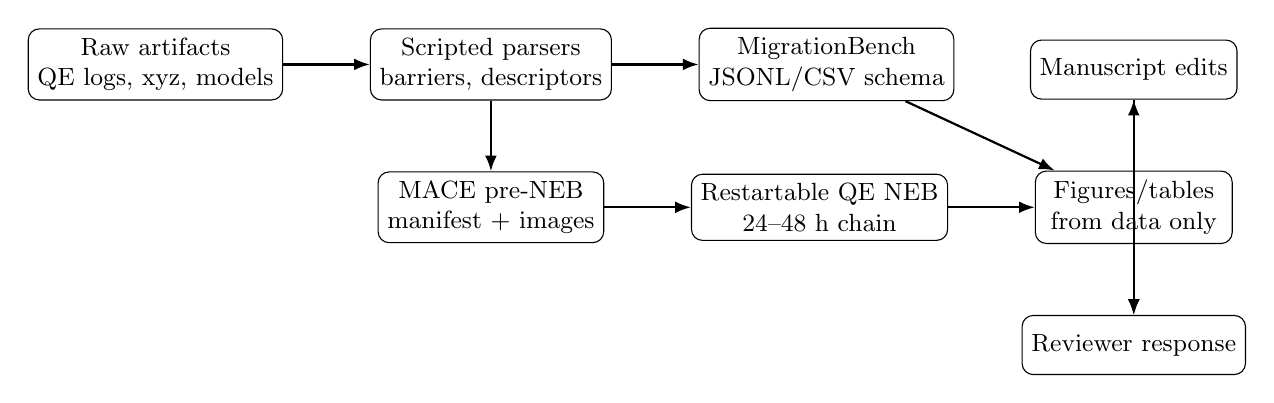
\begin{tikzpicture}[
    node distance=0.9cm and 1.1cm,
    box/.style={draw,rounded corners,align=center,minimum width=2.5cm,minimum height=0.75cm,font=\small},
    arrow/.style={-{Latex[length=2mm]},thick}
  ]
    \node[box] (raw) {Raw artifacts\\QE logs, xyz, models};
    \node[box,right=of raw] (parse) {Scripted parsers\\barriers, descriptors};
    \node[box,right=of parse] (dataset) {MigrationBench\\JSONL/CSV schema};
    \node[box,below=of parse] (mace) {MACE pre-NEB\\manifest + images};
    \node[box,right=of mace] (qe) {Restartable QE NEB\\24--48 h chain};
    \node[box,right=of qe] (figs) {Figures/tables\\from data only};
    \node[box,above=of figs] (paper) {Manuscript edits};
    \node[box,below=of figs] (resp) {Reviewer response};

    \draw[arrow] (raw) -- (parse);
    \draw[arrow] (parse) -- (dataset);
    \draw[arrow] (parse) -- (mace);
    \draw[arrow] (mace) -- (qe);
    \draw[arrow] (qe) -- (figs);
    \draw[arrow] (dataset) -- (figs);
    \draw[arrow] (figs) -- (paper);
    \draw[arrow] (figs) -- (resp);
    \draw[arrow] (paper) -- (resp);
  \end{tikzpicture}
\end{frame}

\begin{frame}{Restartable QE NEB Closure Plan}
  Each long segment obeys:
  \[
  T_{\mathrm{QE,max}} = T_{\mathrm{Slurm}} - T_{\mathrm{safety}}.
  \]

  \begin{table}
  \centering
  \small
  \begin{tabular}{lcc}
  \toprule
  Slurm walltime & Safety margin & QE max\_seconds \\
  \midrule
  24 h & 1800 s & 84600 s \\
  48 h & 1800 s & 171000 s \\
  \bottomrule
  \end{tabular}
  \end{table}

  \vspace{0.2cm}
  Restart loop:
  \[
  \Gamma^{(0)}_{\mathrm{MACE}}
  \rightarrow
  \Gamma^{(1)}_{\mathrm{QE}}
  \rightarrow
  \Gamma^{(2)}_{\mathrm{QE}}
  \rightarrow
  \cdots
  \rightarrow
  \Gdft.
  \]

  Stop when max image error $\le 0.03$ eV/\AA{} and barrier drift $<0.02$ eV.
\end{frame}

\begin{frame}{What Is Still Placeholder}
  \begin{table}
  \centering
  \small
  \begin{tabular}{lll}
  \toprule
  Placeholder & Needed for & Upstream action \\
  \midrule
  Final 1-7 DFT NEB barrier & A1, Fig. 3/SI & long restartable QE chain \\
  Deep-penetration DFT reference & A3, Table S1 & select path and converge QE NEB \\
  SOAP/RMSD overlap minima & A2 & nearest-neighbor audit \\
  Multi-seed mean $\pm$ std & A3/A5 & grouped-split retraining \\
  Corrected FT-600K MD transport & C9/Fig. 2 & rerun corrected MD protocol \\
  SHAP perturbation result & A6/Fig. 6 & cluster perturbation or claim weakening \\
  \bottomrule
  \end{tabular}
  \end{table}

  \vspace{0.2cm}
  Placeholders are not failures; they are explicit guards against unsupported claims.
\end{frame}

\begin{frame}{Final Manuscript Narrative}
  \begin{enumerate}
    \item Equilibrium MLFF metrics are necessary but not sufficient.
    \item Migration and sliding induce non-equilibrium distribution shift.
    \item NEB paths define a task-relevant probe distribution $\Dne$.
    \item Fixed-path and self-relaxed evaluations expose different failure modes.
    \item Fine-tuning changes model bias: local fidelity can improve while global response must be checked.
    \item The revision reports a scoped, auditable benchmark framework rather than overclaiming universal generality.
  \end{enumerate}

  \vspace{0.25cm}
  \begin{block}{Take-home}
  The paper's contribution is a formal diagnostic framework for MLFF deployment risk under non-equilibrium material tasks.
  \end{block}
\end{frame}

\begin{frame}{Discussion Slide}
  \Large
  \[
  \boxed{
  \text{Do we trust a force field because it fits equilibrium data,}
  }
  \]

  \vspace{0.2cm}
  \Large
  \[
  \boxed{
  \text{or because it survives the path the material actually takes?}
  }
  \]

  \vspace{0.5cm}
  \normalsize
  Revision 1 turns the answer into an auditable DAG: data, metrics, figures, and reviewer responses all share the same upstream provenance.
\end{frame}

\end{document}
